%%%%%%%%%%%%%%%%%%%%%%%%%%%%%%%%%%%%%%%
%%%                                 %%%
%%%    The paper about the G-Prop:  %%%
%%%      Genetic Algorithm for      %%%
%%%       Training Perceptrons      %%%
%%%                                 %%%
%%%%%%%%%%%%%%%%%%%%%%%%%%%%%%%%%%%%%%%
\documentclass{elsart}

\usepackage{graphics}
%\def\CC{{C\hspace{-.05em}\raisebox{.4ex}{\tiny\bf ++}}~}
%\addtolength{\textfloatsep}{-0.5cm}
%\addtolength{\intextsep}{-0.5cm}

\begin{document}
\begin{frontmatter}
\title{G-Prop: Global Optimization of Multilayer Perceptrons using GAs}
\author[ugr]{P.A. Castillo}
\author[ugr]{, J.J. Merelo}
\author[ugr]{, A. Prieto}
\author[ujaen]{, V. Rivas}
\author[ugr]{G. Romero}

\address[ugr]{Departamento de Arquitectura y Tecnolog\'{\i}a de Computadoras,
           Facultad de Ciencias, Campus Fuentenueva, s/n, E. 18071,
           Universidad de Granada (Spain),
           {\tt todos@geneura.ugr.es, http://geneura.ugr.es}}
\address[ujaen]{Departamento de Inform\'{a}tica de la Universidad de Ja\'{e}n,
	Escuela Polit\'{e}cnica Superior, Universidad de Ja\'{e}n,
	Avda. Madrid, 35, E. 23071, Ja\'{e}n (Spain) }

 
%%%%%%%%%%%%%%%% abstract %%%%%%%%%%%%%%%
\begin{abstract} 
A general problem in model selection is to obtain the right parameters that make a model fit observed data. For a Multilayer Perceptron (MLP) trained with Backpropagation (BP), this means finding appropiate layer size and initial weights.
This paper proposes a method (G-Prop, genetic backpropagation) that attempts to solve that problem by combining a genetic algorithm (GA) and BP to train MLPs with a single hidden layer. The GA selects the initial weights and changes the number of neurons in the hidden layer through the application of specific genetic operators. G-Prop combines the advantages of the global search performed by the GA over the MLP parameter space and the local search of the BP algorithm. 

The application of the G-Prop algorithm to several real-world and benchmark problems shows that MLPs evolved using G-Prop are smaller and achieve a higher level of generalization than other perceptron training algorithms, such as QuickPropagation or RPROP, and other evolutive algorithms, such as G-LVQ.

\textbf{Keywords}: Genetic Algorithms, Neural Networks, Optimization, Learning, Generalisation
\end{abstract} 

\end{frontmatter}
 

%%%%%%%%%%%%%%%% Introduction %%%%%%%%%%%%%%%
\section{Introduction and State of the Art}
\label{sec:intro}

Using artificial neural networks (ANNs) requires establishing the structure in layers and connections between them, the parameters (such as initial weights) and a set of learning constants. 
As training mechanism, an iterative gradient descent algorithm designed to step by step minimize the difference between the actual output vector of the network and the desired output vector, such as BP in its different versions (like, for instance QuickProp by Fahlman et al.\cite{FahlmanQP}, and RPROP by Riedmiller and Braun \cite{Riedmiller93,Riedmiller94}) is widely used as training mechanism, as well as other evolutionary approaches \cite{competitiveNNGA,Castillo2,Yao98,Yao98b,Miller}.
However, even as these BP methods are successfully used in many fields, especially for pattern recognition, due to its learning ability, it does encounter certain difficulties in practice:
1) convergence tends to be extremely slow and very dependent on the initial weights; 2) convergence to the global optimum is not guaranteed; 3) learning constants and hidden layer size must be guessed heuristically or through systematic tests.

Convergence can be sped up through the use of gradient following techniques \cite{FahlmanCASCOR,Riedmiller93}, but 2) and 3) are more different to tackle, specially since the learning parameters and network size depend on the problem to solve.
Thus the problem of automatic MLP parameter setting and optimization remains an open question.

There are two ways of approaching the optimization of BP parameters for certain problem: Incremental / decremental (see \cite{Alpaydim}, by Alpaydim et al. for an interesting review) or genetic algorithms (see either Yao \cite{Yao92,Yao93} or Balakrishnan et al. \cite{balakrishnan95:EDNA} for an interesting review).


\begin{itemize}
      \item \emph{Incremental algorithms}, such as \emph{Cascade Correlation} by Fahlman and Lebi\`{e}re \cite{FahlmanCASCOR}, and the \emph{Tiling and Perceptron Cascade Algorithm} presented by Parekh et al. in \cite{Parekh}, are based on adding hidden neurons to a network of minimum size until it reaches the required precision.
A sequential orthogonal approach to the building and training of single hidden layer neural networks is also presented by Zhang in \cite{Zhang}. This method starts with a single hidden neuron and increases its number until the error is sufficiently small, or as in the method proposed by Rathbun et al. \cite{Rathbun} constructs MLP from scratch, adding hidden units until the algorithm achieves the required accuracy, there is also a method to prune the network.
One problem of these methods is that once the hidden neurons have been added they cannot be suppressed to reduce the size (the redundant information stored in the weights is never eliminated) and huge ANNs are usually obtained. Furthermore, since weights of existing neurons are frozen, added ones are usually inefficient feature detectors, so the algorithm has to add even more units to improve the obtained results. In general, adding new units lead to overfitting: J. Hwang et al. demonstrated in \cite{Hwang} that the Cascade Correlation algorithm does not generalize well in some classification and regresion problems.

      \item \emph{Decremental algorithms}, such as those presented by Jasic et al. in \cite{Jasic} and Pelillo et al. in \cite{Pelillo}, usually called pruning methods, are based on taking a network with an initially high number of connections, and then eliminating them one by one, to obtain a smaller network but with the same (or better) classification ability.
These algorithms work by searching redundant noncontributing or duplicate nodes.
After pruning, ANN must usually be re-trained. The problem with these methods is that they start with excessively big networks, which slows down training. However, depending on the selection criteria used to select the neurons to be pruned, it is possible to obtain a good solution, if the right units to eliminate and the elimination order are guessed correctly.
Another approach is to set some of the weights to zero as is done in \emph{Optimal Brain Damage}, by Le Cun et al. \cite{LeCun}, and \emph{Optimal Brain Surgeon}, by Hassibi et al. \cite{Hassibi}. The problem presented by this method is that near co-linearities can mean that if one weight is set to zero, the standard errors for the others are drastically reduced, so it may be unsafe to set more than one weight to zero at a time. 
Both decremental and incremental algorithms are gradient descent optimization methods, so they suffer the problem that they may reach the closest local minimum to the search space point where the method began.\\
\end{itemize}

\emph{Evolutionary neural networks} provide an alternative for this task of controlling the complexity by adjusting the number of weights of the ANN. They are an example of a \emph{hybrid aproach} of a GA and BP to train ANN. 
The Baldwin effect may arise in evolutionary computation when a genetic algorithm is used to evolve a population of individuals that also employ a local search algorithm (Hinton and Nowlan \cite{Hinton}). In computational terms, in a first step of the Baldwin effect, local search smooths the fitness landscape, which can facilitate evolutionary search. In a second step, as more optimal individuals arise in the population, there is selective pressure for reduction in local search, driven by the intrinsic costs associated with the search.
GAs can be applied to design ANN in several ways \cite{Yao92,Marin95}:

\begin{itemize}
      \item \emph{Search for the optimal set of weights} of a pre-established topology net, as did Topchy et al. in \cite{Topchy}, where a GA is used to evolve a population of ANN by encoding the parameters of the hidden layer into binary strings. This approach uses a pre-established connectivity and number of neurons, and it does not allow to search other topologies.  De Falco et al. propose a method \cite{FalcoPPSN98} based on an evolutionary approach to provide the optimal set of synaptic weights of the network. 
Some authors use binary encoding of weights into individuals (Whitley et al. \cite{Whitley93}) while others use dynamic encoding, like Gray encoding (Schraudolph and Belew \cite{Schraudolph92}).
Keesing and Stork \cite{Keesing} proposed a method that combines a GA and neural networks to solve a simple pattern recognition problem, which takes advantage of the Baldwin effect \cite{Baldwin} to increase the rate of evolution: too little of too much learning leads to poorer evolution than does an intermediate amount of learning.
Main problem with this approach is that it concentrates on optimizing only a part of the neural net, disregarding the rest: hidden layer size and learning constants.

      \item \emph{Search over topology space}, as did White et al. in \cite{White}, where a GA, using a population initialized with different hidden layer sizes, is presented. In this approach, each individual is a complete neural network, and the allele is a hidden or output node with its associated input links. The main problem of this method is that it only search using sizes obtained during the initialization phase. Another method to determine the architecture is presented by Miller et al. in  \cite{Miller}, where the network connection structure is mapped onto a binary adjacency matrix called \emph{Miller-Matrix} (MM) describing ANN architecture, but matrix representation of the network: it can generate incorrect network structures (feedback connections) and very long codes for larger networks and it works only with fixed size nets. Bebis et al. \cite{Bebis} propose the coupling of GAs with weight elimination (by Weigend et al. \cite{Weigend}) to search the architecture by pruning oversized networks. This method begins with big networks and, using the GA, searches for the best set of parameters to apply the weight elimination method. 
The method proposed by Yao and Liu \cite{Yao98,Yao98b} combines the search for the optimal set of weights and the search for the optimal topology of modular neural nets. They use a GA to evolve individual modules and integrate them in the same evolutionary process.
De Falco et al. present a method \cite{Falco2} based on an evolutionary approach to face the optimization of the design of a neural network architecture and the choice of the best learning method.
A problem of using a matrix representation is that some networks can generate big individuals. To avoid this problem, some methods of indirect coding have been proposed, as did Kitano \cite{Kitano90}, Harp et al. \cite{Harp89}, Dodd et al. \cite{Dodd91} and Gruau \cite{Gruau92}.

      \item \emph{Search for the optimal learning parameters}, including weights, having pre-established the number of neurons and the connectivity between them, as did Merelo et al. in \cite{competitiveNNGA}, for multilayer competitive learning neural nets, where a method that codifies the weights and learning parameters onto chromosomes is presented. Another example is the method presented by Petridis et al. in \cite{Petridis} where both weights and learning parameters are represented as bit strings to be evolved. Another approach that searches for the learning parameters of the net, based on Simulated Annealing is proposed by Castillo et al. in \cite{Castillo2}.
      \item \emph{Genetic approaches} that modify the BP algorithm, as did Kinnebrock in \cite{Kinnebrock}, where a mutation operator that adds or substracts an amount to the weight values after each iteration is presented. The disadvantage of this method is that such modifications do not necessarily improve the net classification error.
\end{itemize}

Both decremental and incremental algorithms are gradient descent optimization methods, so they suffer the problem that they may reach the closest local minimum to the search space point where the method began.
Evolutionary neural networks are a more efficient way of searching, but still, they search over a subset of all possible parameters.

The aim of this paper is to present an algorithm that searches over the initial weights and hidden layer size of a MLP, based on a GA and BP. It will be proved that it obtains better results than the BP alone, and it only needs to set the learning constant by hand (it obviously needs to set GA constants, but is robust enough to obtain good results under the default parameter settings).
We intend to make use of the capacity of both algorithms: the ability of the GA to find a solution close to the global optimum, and the ability of the BP to tune a solution and reach the nearest local minimum by means of local search from the solution found by the GA.
Instead of using a pre-established topology, the population is initialized with different hidden layer sizes, with some specific operators designed to change it.
As genetic operators, mutation, multi-point crossover, addition, elimination and substitution of hidden units have been selected.
Thus, the GA searches and optimizes the architecture (number of hidden units) and the initial weight setting for that architecture.
Unlike other approaches \cite{Yao98}, the hidden layer maximum size is not bounded in advance.


G-Prop main contributions to the field of neurocomputing are: 
\begin{itemize}
      \item A GA is applied directly to a population of MLP, instead of some codification of the network. Thus a lineal or binary representation is not needed in order to evolve the population.
      \item GA is used to modify the initial weights only, while BP is used to train from those weights. This makes a clean division between global and local search.
      \item The hidden layer size is searched throught the aplication of some new GA operators: substitution, addition and elimination. These operators are developed to perform incremental (adding hidden neurons) or decremental (pruning hidden neurons) learning.
      \item The program does not takes much more time than plain BP to find a better solution.
\end{itemize}


The remainder of this paper is structured as follows: Section \ref{sec:method} presents the G-Prop algorithm, followed by the architecture and genetic operators. Section \ref{sec:expe} describes the results obtained, followed by a brief conclusion in Section \ref{sec:conclus}.
 

%%%%%%%%%%%%%%%% Method %%%%%%%%%%%%%%%
\section{The genetic algorithm in G-Prop}
\label{sec:method}

The designed algorithm is specified in the following pseudocode:

\begin{enumerate} 
	\item Generate the initial population with random weight values and hidden layer sizes uniformly distributed from 2 to a maximum of MAX (this is needed in order to have a diversity of sizes).
	\item Repeat for $g$ generations:
		\begin{enumerate} 
			\item Evaluate the new individuals: train them using the training set and obtain their fitness according to the number of correct classifications on the validation set and the hidden layer size.
			\item Select the $n$ best individuals in the population, according to their fitness, and mate them, using mutation, crossover, addition, elimination and substitution of hidden neurons.
			\item Replace the $n$ worst individuals by the new ones.
		\end{enumerate} 
	\item Use the best individual to obtain the testing error.
\end{enumerate} 

The classification accuracy or number of hits is obtained by dividing the number of hits between the total number of examples in the testing set.
In G-Prop the \emph{fitness function} is given by the number of hits when carrying out the test after the training, and in the case of two individuals with identical classification error (measured as the number of elements incorrectly classified) the best is the one that has a hidden layer with fewer neurons. This implies greater speed when training and classifying and facilitates its hardware implementation; besides, it improves generalization. 

A \emph{steady state} \cite{Whitley} algorithm was used because it was empirically found to be faster at obtaining solutions than other selection algorithms. For each generation, the best $n$ individuals of the population, those whose fitness is highest, are chosen to mate, using the genetic operators. The offspring replace the $n$ worst individuals of the current generation.


In principle, evolved MLPs should be codified into chromosomes to be handled by the genetics operators of the GA. But G-Prop uses no binary codification; instead, the initial parameters of the network are evolved using specific genetic operators (see below), such as mutation, crossover and the substitution, addition and elimination of hidden neurons: this is made possible by the \textbf{EO} (Evolvable$|$Evolutionary Objects) library philosophy (see next section), according to which any object with a fitness can be evolved. Moreover, this agrees with the spirit of Z. Michalewicz: Genetic Algorithm plus Data Structures equal Evolution Programs \cite{Michalewicz} . The genetic operators act directly on the ANN object, but only \emph{initial weights} are subjected to evolution, not the weights obtained after training (a clone of the MLP is created and trained to compute its fitness function, thus the initial weights remain unchanged in the original MLP). The ``genetic atom'' is a hidden layer neuron; most operators deal with hidden layer neurons and weights to and from it as an unit.

Five genetic operators are used to change MLP. Besides the percentage of mutation and the number of crossing points, the application priority for each operator has to be specified to indicate the number of individuals generated by each genetic operator. The tests have been done using a higher priority for mutation and the same level for the remaining operators. 
\begin{itemize}

\item The \emph{mutation} operator modifies the weights of certain neurons, at random, depending on the application rate. It is based on the algorithm presented in \cite{Kinnebrock}, which modifies the weights of the network after each epoch of network training, adding or subtracting a small random number that follows \emph{uniform} distribution with the interval $[-0.1,0.1]$.
This operator was used with an application probability of $40\%$, that is, $40\%$ of weights are changed, which was found empirically to obtain better results than did lower probabilities.

\item The \emph{CrossOver} operator carries out the multipoint cross-over between two chromosome nets, so that two networks are obtained whose hidden layer neurons are a mixture of the hidden layer neurons of both parents: some hidden neurons along with their \emph{in} and \emph{out} connections, from each parent make one offspring and the remaining hidden neurons make the other one.

\item The \emph{Addition} operator and the following (Elimination) attempt to solve one of the main problems of BP and its variants: the difficulty in guessing the number of the hidden layer neurons. By adding hidden neurons it is not necessary to set the size of the GA search space.
This operator is intended to perform incremental learning: it starts with a small structure and increments it, if neccesary, adding new hidden units. 
At the same time, it raises the dilemma of overfitting: small networks generalize well, but they are slow learning, whereas big networks are fast learning, but generalize badly \cite{Bellido,Bebis}.

\item The \emph{Elimination} operator eliminates one hidden neuron at random. This operator is intended to perform decremental learning: it prunes certain nodes to obtain better results in generalization and a smaller network \cite{Jasic,Pelillo,Bebis}. Thus, to a certain extent, the networks are prevented from growing too much.

\item The \emph{Substitution} operator is applied at a low priority and replaces one hidden layer neuron at random with a new one, initialized with random weights. This operator may be considered a kind of mutation that affects only one gene.

\end{itemize}

The algorithm was run for a fixed number of generations.
When evaluating each individual of the population to obtain its fitness a limit of epochs was established. 


We have used the BP variant known as the perceptron training algorithm \emph{QuickProp} \cite{FahlmanQP}. This algorithm, together with RPROP \cite{Riedmiller93,Riedmiller94} BP variant, is one of the best avoiding local minima (one of the problems of BP) because the magnitude of the change in the weights (the step size) is not a function of the magnitude of the gradient.
The QuickProp algorithm, together with GA, improves the probability of avoiding local minima.
 

%%%%%%%%%%%%%%%% experiments and results %%%%%%%%%%%%%%%
\section{Experiments and results}
\label{sec:expe}

We used \textbf{EO} library as a toolbox to develop G-Prop, due to the facility that this library offers to evolve any object with a fitness function and use anything as a genetic operator. EO is a C++ toolbox which defines interfaces for many classes of algorithms used in evolutionary computation and, at the same time, provides some examples that use those interfaces. It is available at \emph{http://geneura.ugr.es/\symbol{126}jmerelo/EO.html}. One of the objectives of using EO is to make it easier to reproduce results, which is why the source for all objects evolved with EO should also be made available, together with the articles that mention them. G-Prop is available at \emph{http://geneura.ugr.es/\symbol{126}pedro/G-Prop.htm}

First, the dynamics of G-Prop as a genetic algorithm are shown and then compared with other methods.
The evolution of classification accuracy and hidden layer size during a typical run are shown in figure  \ref{fig:graf} , usually, each of these quantities is usually optimized in turn: classification accuracy is optimized first, since it is given higher priority in fitness evaluation; then, while keeping the same classification accuracy, G-Prop optimizes size. 

In the run shown here, in generation 1, a MLP with the same classification accuracy ($97.7\%$) but fewer hidden neurons (3) is found; at generation 2, a perceptron with better classification accuracy ($98.2\%$) but more hidden neurons (4) is found; later on during the simulation, a perceptron with the same accuracy but fewer hidden neurons (3) is selected as the winner.

G-Prop was run 20 times with the same parameter settings and a different random initialization for each benchmark used.

%las graficas...
\begin{figure}
\begin{center}
\begin{tabular}{cc}
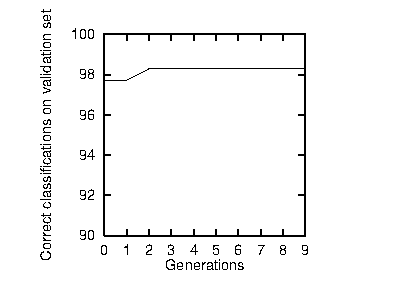
\includegraphics{hit.eps} & 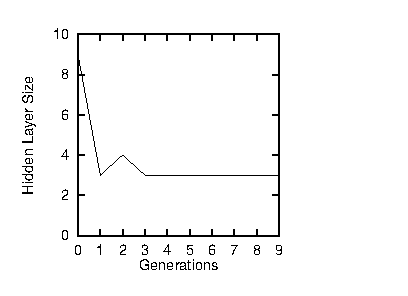
\includegraphics{size.eps} \\
a & b
\end{tabular}
\caption{\small{Evolution of the classification accuracy of G-Prop in terms of hits percentage (a) and of the hidden layer size (b) during a typical run. At generation 1, a MLP with same classification accuracy ($97.7\%$) but fewer hidden neurons (3) is found; at generation 2, a perceptron with better accuracy ($98.2\%$) but more hidden neurons (4) is found; later on during the simulation a perceptron with the same accuracy but fewer hidden neurons (3) takes its place.}}
\label{fig:graf}
\end{center}
\end{figure}

The tests used to assess the accuracy of G-Prop and other must be chosen carefully, because some tests (exclusive-or problem) are not suitable for certain capacities of the BP algorithm, such as generalization \cite{FahlmanBENCHMARKS}. Our opinion, along with Prechelt \cite{Prechelt94c}, is that to test an algorithm, at least two real world problems should be used.
This is why comparisons with other GA+NN algorithms are not included in this paper: in other published papers \cite{White,Miller,Kitano90,Gruau92}, they were applied to toy or non public available problems.

The tests were applied as follows: each data set was divided into three disjoint parts, for training, validating and testing. Thus, in order to obtain the fitness of an individual, the MLP is trained with the training set and its fitness is established from the classification error with the validating set. 
Once the GA is finished (when it reaches the limit of generations), the classification error with the testing set is calculated this is the shown result.

To obtain the results with the program that implements QP, the methodology used was to train as many MLPs as were trained by G-Prop on a run (about 120 MLPs), using the \emph{same topology} of the best net found by the proposed method, for a particular benchmark. Then the validating set is used to obtain the validating error for each MLP; once the best MLP is found, the testing error is obtained on the testing set. 
The results which have an error greater than five times the error average are not taken into account to obtain the final results.
The RPROP results, quoted here come from Prechelt \cite{Prechelt94c}. 
The basic principle of Rprop is to eliminate the influence of the size of the partial derivative on the weight step. As a consequence, only the sign of the derivative is considered to indicate the direction of the weight update.


\emph{Cancer.}
This dataset is from the UCI machine learning dataset "Wisconsin breast cancer database". This breast cancer database was obtained from the University of Wisconsin  Hospitals, Madison from Dr. William H. Wolberg \cite{Wolberg}.
An exhaustive report, by Prechelt, on this dataset (and others) is given in \cite{Prechelt94c}.
Each sample has 10 attributes plus the class attribute: Sample code number, Clump Thickness, Uniformity of Cell Size, Uniformity of Cell Shape, Marginal Adhesion, Single Epithelial Cell Size, Bare Nuclei, Bland Chromatin, Normal Nucleoli, Mitoses, Class (0 for benign, 1 for malignant).
The class distribution in the original set is the following: $65.5\%$ Benign and $34.5\%$ Malignant.

\emph{DNA Helicases.}This is a problem of electron microscopy image classification. The object of the classification is to study the structure of a representative hexametric helicase: the large T antigen of Simian Virus 40 \cite{Tantigen}. When observed in the electron microscope, large T antigen preparations mainly show either a characteristic roughly circular view with a stain penetrating region in the centre (which we will call a top view) or a view with a rectangular shape (side view).
This training/test set has been used in \cite{heliNPL} to classify images of the large T antigen of Simian Virus 40.
The set consists of 197 examples, divided into the training set (78 examples), validating set (60) and testing set (59).
Each example consists of 25 inputs (the 25 blocks of the image to be classified), and the output: 0 is side view and 1 is top view.

The tests were carried out, using the described benchmarks, with our own version of QP (available as part of the G-Prop package) and the proposed method, G-Prop.

For the \emph{Cancer} problem the GA was executed for 10 generations on a population of 20 individuals (neither too many generations nor a very large population, in order to avoid long runs), with a mutation probability of 0.5 (which was found empirically to generate better individuals than a lower probability) and 2 crossing points for the crossover operator. In each generation, $50\%$ of the population is replaced by new individuals (to prevent the population from remaining too static and perhaps not evolving at all).
The individuals, MLP with 9 inputs, 2 outputs and a number of hidden units between 2 and 20, were evaluated with 100 epochs and a suitable learning coefficient for this problem, where a MLP can easily fall into a local minimum (0.007).
Each execution with these parameters took several minutes.

To show the improvement of a GA over purely random search, the networks were trained for 1000 epochs. 
The results obtained for the first test ($\%$ of error in test), compared with those obtained by Prechelt in \cite{Prechelt94c}, are shown in table \ref{table:cancer}.

\begin{table}
\begin{center}
\begin{tabular}{|c|c|c|c|c|c|}
\hline 
\multicolumn{2}{|c|}{Cancer} & Error$\% \pm$ Std Dev & Hidden Units $\pm$ Std Dev (Parameters)  \\
\hline
\hline
Cancer 1 &   QP     & 17  $\pm$ 17  &   3 (33)  \\
         &          & 13  $\pm$ 16  &   9 (99)  \\
\cline{2-4}
         &   G-Prop &  1.0  $\pm$ 0.5   &  3.2 $\pm$ 0.8 (35.2)  \\
\cline{2-4}
         & Prechelt & 1.149             &   4+2 (48)  \\ %4+2
\hline
\hline
Cancer 2 &   QP     & 15  $\pm$ 14  &  7 (77)   \\
         &          & 27  $\pm$ 13  & 12 (132)  \\
\cline{2-4}
         &   G-Prop & 4.4   $\pm$ 0.4   & 6.7 $\pm$ 2.3 (73.7)  \\
\cline{2-4}
         & Prechelt & 5.747             &  6+6 (112)  \\ %8+4
\hline
\hline
Cancer 3 &   QP     & 13 $\pm$ 15   &   4 (44)  \\
         &          & 18  $\pm$ 17  &   8 (88)  \\
\cline{2-4}
         &   G-Prop & 3.0   $\pm$ 0.7   & 4.3 $\pm$1.7 (47.3)  \\
\cline{2-4}
         & Prechelt & 2.299             & 4+4 (60)  \\ %4+4
\hline

\end{tabular}
\end{center}
\caption{\small{Results of evaluating QP and G-Prop for the Cancer problem. RPROP results are taken from \cite{Prechelt94c}. This table shows the average error rate and the average size of nets, as the number of parameters (number of weights of the MLP) and as the number of hidden units.}}
\label{table:cancer}
\end{table}

In general, G-Prop obtains MLPs with a slightly lower generalization error than other methods (QP and RPROP), except in Cancer 3, for which Prechelt \cite{Prechelt94c}, using the RPROP variation of the BP learning algorithm, presents better results; however he does not mention standard deviation (although G-Prop obtains smaller sized networks, 4.3 neurons, with a similar classification error, $3.0 \pm 0.7$). On average G-Prop is slightly better than RPROP, both in error rates and net size.

Yao and Liu present a method to evolve modular neural networks and the results obtained on the cancer problem in \cite{Yao98b}. However the results they present are better on classification accuracy ($0.037 \pm 0.012$), the network sizes obtained are greater ($13.1 \pm 1.2$) than those obtained using G-Prop. Moreover, we have not included Yao's results in table \ref{table:cancer} because we have used three different cancer sets to test G-Prop against QP and RPROP, while Yao and Liu use only one of them. Thus, although Yao and Liu also use the cancer problem, we do not know against which cancer problem we have to compare to.


For the \emph{DNA helicases} problem, the GA was executed for 10 generations on a population of 20 individuals, with a probability of mutation of 0.5 and 2 crossing points for the crossover operator. Each generation, $50\%$ of the population is replaced by new individuals.
The individuals, MLP with 25 inputs, 2 outputs and a number of hidden units between 2 and 15, were evaluated with 100 epochs and a suitable learning coefficient for this problem, where a MLP can easily fall into a local minimum (0.07).
Each execution with these parameters took several minutes.

Table \ref{table:heli} shows the results obtained with both algorithms and compares them to the ones shown in \cite{heliNPL}.

\begin{table}
\begin{center}
\begin{tabular}{|c|c|c|c|c|}
\hline 
\multicolumn{2}{|c|}{DNA Helicases} & Error$\% \pm$ Std Dev & Hidden Units $\pm$ Std Dev (Parameters)  \\
\hline
\hline
\multicolumn{2}{|c|}{QP}     &  9 $\pm$ 10  &  7 (189)  \\
\multicolumn{2}{|c|}{}       &  9 $\pm$  9  &  11 (297)  \\
\hline
\multicolumn{2}{|c|}{G-Prop} & 6  $\pm$ 3   &  7.3 $\pm$ 3.9 (197.1)  \\
\hline
        &  20 generations &  18   $\pm$   2    &  2.3 $\pm$ 0.4 (59.5) \\
  G-LVQ &  50 generations &  13   $\pm$   3    &  2.2 $\pm$ 0.3 (57) \\
        & 100 generations &  15   $\pm$   5    &  2.2 $\pm$ 0.3 (57)\\
\hline

\end{tabular}
\end{center}
\caption{\small{Results of evaluating QP and G-Prop on the classification of different views of large T antigen of Simian Virus 40, and the results obtained with G-LVQ \cite{heliNPL}.}}
\label{table:heli}
\end{table}

In the \emph{DNA helicases} problem, it is evident that G-Prop outperforms other methods: G-LVQ \cite{heliNPL} takes arround 20 generations to achieve an error of $18 \pm 2$, while G-Prop  achieves an error of $6.10 \pm 3.01$.

As it has been shown, in both problems the standard deviation for the G-Prop algorithm is much smaller than that for QP. This further supports the notion that QP may often be trapped in various different local minima whereas G-Prop can avoid many of such traps. Moreover, Prechelt \cite{Prechelt94c} does not mention the standard deviation value, but it can be seen that G-Prop obtains much smaller values than those obtained using G-LVQ \cite{heliNPL}.

Each run of the proposed method takes about 3 minutes on a Pentium 233MMX, using the parameters described above, while each run of QP takes about 1 minute; thus, it is evident that is less time-consuming apply G-Prop than to train as many randomly-initialized MLPs using QP.

Summing up, these experiments show that G-Prop avoids the task of setting MLP parameters, finding them as a result, and besides, obtains smaller networks and with less error than other procedures.

%%%%%%%%%%%%%%%% conclusions %%%%%%%%%%%%%%%
\section{Conclusions}
\label{sec:conclus}


This paper presents G-Prop, an algorithm to train MLPs based on GA and BP. Experiments prove that the proposed method achieves better results than other non-evolutionary variants and, besides, obtains network size as a result.

In particular, the proposed algorithm (G-Prop) obtains a much higher degree of generalization (that is, error on a previously unseen test set) than that achieved by other BP algorithms such as QP or RPROP, minimizing the number of hidden units as the second optimization criterion.

The idea of the approach presented here is to use an MLP population that will be evaluated to obtain its classification ability. This value, together with the hidden layer size, is used to determine fitness. Using the individuals with highest fitness, after having applied the designed genetic operators, a new population is obtained.

The GA evaluates each individual taking into account the classification capacity and the hidden layer size. The weights of the individuals/nets of the first generation are generated randomly, and these are the weights that the GA will evolve using operators that alter the ANN size. 
This strategy attempts to avoid Lamarckism (i.e., that individuals inherit the trained weights from their parents), but, at the same time, it is a good strategy to avoid local minima.

Several benchmarks (cancer 1, 2 and 3, and DNA helicases) have been used to test the proposed algorithm and to compare it with others \cite{Prechelt94c,heliNPL}. The results show that the GA obtains a MLP whose classification accuracy is better than that obtained by training a MLP using only conventional procedures.

Future work will extend the presented method and will include the development of new genetic operators and the improvement of those described here, to perform incremental learning (\emph{pruning} and \emph{addition} operators) from the approach presented in  \cite{FahlmanCASCOR} and \cite{Pelillo}.
The QP algorithm will also be used as an operator in the GA, as suggested in \cite{Montana}, and it will be used to check the Baldwin effect on the rate of evolution, as it is proposed by Keesing and Stork \cite{Keesing}.
Finally, the presented algorithm will be applied to solve other real world problems.


%%%%%%%%%%%%%%%% acknowledgements %%%%%%%%%%%%%%%
\section{Acknowledgements}
\label{sec:ackn}
This work has been supported in part by the CICYT project BIO96-0895 (Spain), the DGICYT project PB-95-0502 and the FEDER I+D project 1FD97-0439-TEL1.

The authors are grateful to anonymous referees for their constructive comments and advice about the first revision of the paper.


%%%%%%%%%%%%%% Bibliografy %%%%%%%%%%%%%%%
\bibliographystyle{unsrt}
\bibliography{correccion}


\end{document}
